\documentclass[a4paper, 12pt]{report}


% \usepackage[portuges]{babel}
\usepackage[utf8]{inputenc}
\usepackage{amsmath,amssymb}
\usepackage{graphicx}
\usepackage{subfig}
\usepackage{indentfirst}
\usepackage{verbatim}
\usepackage{textcomp}
\usepackage{gensymb}
\usepackage{ragged2e}
\usepackage{relsize}
\usepackage[utf8]{inputenc}
\usepackage{float}

\usepackage{setspace}
\usepackage{titlesec}
\linespread{1.5}   
\NewDocumentCommand{\myrule}{O{1pt} O{2pt} O{black}}{%
  \par\nobreak % don't break a page here
  \kern\the\prevdepth % don't take into account the depth of the preceding line
  \kern#2 % space before the rule
  {\color{#3}\hrule height #1 width\hsize} % the rule
  \kern#2 % space after the rule
  %\nointerlineskip % no additional space after the rule
}
\usepackage[section]{placeins}

\usepackage{booktabs}
\usepackage{colortbl}%
   \newcommand{\myrowcolour}{\rowcolor[black]{0.925}}

\usepackage[obeyspaces]{url}
\usepackage{etoolbox}
\usepackage[colorlinks,citecolor=black,urlcolor=blue,bookmarks=false,hypertexnames=true]{hyperref} 

\usepackage{geometry}
\geometry{
	paper=a4paper, % Change to letterpaper for US letter
	inner=2cm, % Inner margin
	outer=2cm, % Outer margin
	bindingoffset=.5cm, % Binding offset
	top=2cm, % Top margin
	bottom=2cm, % Bottom margin
	%showframe, % Uncomment to show how the type block is set on the page
}


\begin{document} 

%************************************TITLE PAGE**************************************%
\begin{titlepage}
\begin{center}
\textbf{\LARGE Tribhuvan University}\\[0.5cm] 
\textbf{\large Institute of Science and Technology}\\[0.2cm]
\vspace{20pt}\includegraphics[width=10cm]{images/Logo.png}\\
\par
\vspace{15pt}
  \textbf{\Large Central Department of Computer Science and Information Technology}\\
  Kirtipur, Kathmandu\\
\vspace{15pt}  
\centering
\rule[10pt]{1.5pt}{60pt}
\rule[0pt]{1.5pt}{80pt}
\rule[10pt]{1.5pt}{60pt}\\
\begin{center}
\textbf{In partial fulfillment of the requirement for Master’s Degree in Computer Science and Information Technology (M.Sc. CSIT), Second Semester}\\
\end{center}
\textbf{\LARGE  Seminar Report on:}\\ [0.2cm]

\textbf{\large “Comparative Analysis of Word Embedding Models for Nepali Text Classification"}\\
\vspace{15pt} 
\textbf {\large Submitted To:}\\[0.2cm]
\textbf {Central Department of Computer Science and Information Technology}\\[0.1cm]
\vspace{15pt}  
\textbf {\large Submitted By:}\\[0.2cm]
\textbf{Sudhan Kandel (623/077)}\\[0.1cm]
\text{August, 2022 }
\end{center}
\par
\vfill

\end{titlepage}
\newpage
\pagenumbering{gobble}
%************************************SUPERVISOR RECOMMENDATION PAGE**************************************%
\pagenumbering{roman}
\begin{center}

\vspace{70pt}\includegraphics[width=10cm]{images/Logo.png}\\
\textbf{\LARGE Tribhuvan University}\\[0.5cm]
\textbf{\large Institute of Science and Technology}\\[0.2cm]
\vspace{40pt}
\textbf{\large Supervisor’s Recommendation}\\
\end{center}
\justifying
I hereby recommend that this Seminar report, prepared under my supervision by \textbf{Mr. Sudhan Kandel} entitled \textbf{“Performance Analysis of Word Embedding Models for Nepali Text Classification”} be accepted as fulfillment in partial requirement for the degree of Master’s of Science in Computer Science and Information Technology. To the best of my knowledge, this is an original work in computer science. 
\vspace{70pt}

\begin{center}
\vspace{25mm}

\begin{tabular}{@{}p{2.5in}@{}}
\hrulefill \\
\centering  Asst. Prof. Bikash Balami\\
\centering Central Department of Computer Science and Information Technology
\end{tabular}
\end{center}

%************************************letter of approval**************************************%
\clearpage
\vspace{70pt} 
\begin{center}
\textbf{\LARGE Tribhuvan University}\\[0.5cm]
\textbf{\large Institute of Science and Technology}\\[0.2cm]
\vspace{30pt}
\textbf{LETTER OF APPROVAL}
\end{center}
This is to certify that the seminar report prepared by \textbf{Mr. Sudhan Kandel} entitled \textbf{“Performance Analysis of Word Embedding Models for Nepali Text Classification”} in partial fulfillment of the requirements for the degree of Master of Science in Computer Science and Information Technology has been well studied. In our opinion, it is satisfactory in the scope and quality as a project for the required degree. \\
\begin{center}
\begin{tabular}{@{}p{2.5in}p{2in}p{2in}@{}}
\hrulefill && \hrulefill\\
Asst. Prof. Sarbin Sayami &&   Asst. Prof. Bikash Balami\\
(HOD) &&  (Supervisor)\\
Central Department of Computer Science and Information Technology &&Central Department of Computer Science and Information Technology
\end{tabular}
\end{center}
\begin{center}
\vspace{25mm}

\begin{tabular}{@{}p{2.5in}@{}}
\hrulefill \\
\centering (Internal)
\end{tabular}
\end{center}


%************************************Acknoledgement**************************************%

\newpage

\begin{center}
\textbf{\LARGE ACKNOWLEDGEMENT}
\addcontentsline{toc}{chapter}{\numberline{} ACKNOWLEDGEMENT}%
\end{center}
\vspace{20pt}
The success and final outcome of this seminar report required a lot of guidance and assistance from many people and I am very fortunate to have got this all along the completion. I am very glad to express my deepest sense of gratitude and sincere thanks to my highly respected and esteemed supervisor \textbf{Asst. Prof. Bikash Balami} Central Department of computer science and Information Technology for his valuable supervision, guidance, encouragement, and support for completing this seminar report. 
I am also thankful to \textbf{Asst. Prof. Sarbin Sayami}, HOD of Central Department of Computer Science and Information Technology for his constant support throughout the period.
Furthermore, with immense pleasure, I submit by deepest gratitude to the Central Department of Computer Science and Information Technology, Tribhuvan University, and all the faculty members of CDCSIT for providing the platform to explore the knowledge of interest. At the end I would like to express my sincere thanks to all my friends and others who helped me directly or indirectly. \\\\
\vspace{50pt}
\textbf{Sudhan Kandel (623/077) }

%************************************Abstract**************************************%
\clearpage
\begin{center}
\textbf{\LARGE ABSTRACT}
\addcontentsline{toc}{chapter}{\numberline{} ABSTRACT}%
\end{center}
\vspace{20pt}
The task of classifying unstructured document to the proper category to which it belongs to is become difficult task because the volume of information shared over the internet increase swiftly. Text classification is the task of allocating the document into one or more number of predefined categories. Additionally, this is very famous in the field of information retrieval, text summarization and so on. However, all the application areas transformation of text into feature vectors play the important role.Previously several text representation techniques have been proposed by different authors to capture the real semantics of the web documents, but this has become hinderance because of semantic mismatch and multiple meanings of words.\\
Thus, this seminar report proposes a word embedding to solve the document representation problem in Nepali news classification. To achieve this task, this seminar work utilizes Word2Vec and ELMo word embedding algorithms to represent documents. And which are also used in conjunction with Nepali news classification algorithm to determine the most effective embedding model. In this report two machine learning algorithm namely SVM and Random Forest are used.\\
Context dependent and independent word representation model are used in this seminar report. Here total of 5145 Nepali news is scraped from e-kantipur for analyzing these models with text classification model, to which it includes four different categories. All in all, the Random Forest machine learning algorithm provide the highest accuracy of 74 percent with the ELMo word representation. However, scenario with SVM looks different, it gives the highest accuracy of 68 percent with Word2Vec word vectorization model.\\
\textbf{Keywords:}
\textit{Word2Vec, ELMo, Word-Embedding}


%************************************TABLE OF CONTENT**************************************%
\hypersetup{linkcolor=black}
\tableofcontents
\addcontentsline{toc}{chapter}{\numberline{} Table of Content}%

  

%*********************List of Figures**********%
\listoffigures
\addcontentsline{toc}{chapter}{\numberline{} List of Figures}%
%*********************List of table**********%
\listoftables
\addcontentsline{toc}{chapter}{\numberline{} List of Tables}%

%*********************List of Abbreviations**********%
\clearpage
\begin{center}
\textbf{\LARGE List of Abbreviations}\\
\addcontentsline{toc}{chapter}{\numberline{} Abbreviations}%
\end{center}
\begin{itemize}
  \item {\textbf{HTML: Hyper Text Markup Language}}
  \item{\textbf{LSTM: Long Short Term Memory}}
  \item{\textbf{NLP: Natural Language Processing}}
  \item {\textbf{NLTK: Natural Language Processing}}
  \item {\textbf{PCA: Principal Component Analysis}}
  \item{\textbf{SBD: Sentence Boundary Disambiguation}}
 \item{\textbf{SOTA: State of The Art }}
  \item{\textbf{SVM: Support Vector Machine}}
\end{itemize}
  
%********************************%
%***********SECTION 1************%
%********************************%
\newpage
\pagenumbering{arabic}
\chapter{INTRODUCTION}
\section{Overview}
\vspace{20pt}
Text classification is a construction problem of models which can classify new documents into pre-defined classes. It involves assigning documents into their predefined categories based on their contents. In many real-world scenarios, the ability to automatically classify documents into a fixed set of categories is highly desirable. This allows users to find desired information faster by searching only the relevant categories and not the entire information space. The importance of text classification is even more apparent when the information space is huge such as the World Wide Web \cite{ajose2020performance}.\\
Word embedding is a way to represent a word with fixed-length vector of continuous real numbers. It maps a word in a vocabulary to a latent vector space where words with similar context are in proximity. Through word embedding, a word is converted to a vector that summaries both the word’s syntactic and semantic information. Consequently, word embedding is particularly suitable to be used as feature representations in neural network model for downstream natural language processing task, such as text classification, machine translation, sequence learning \cite{bhoir2017comparative}.\\
\begin{figure}
  \centering 
  \vspace{20pt}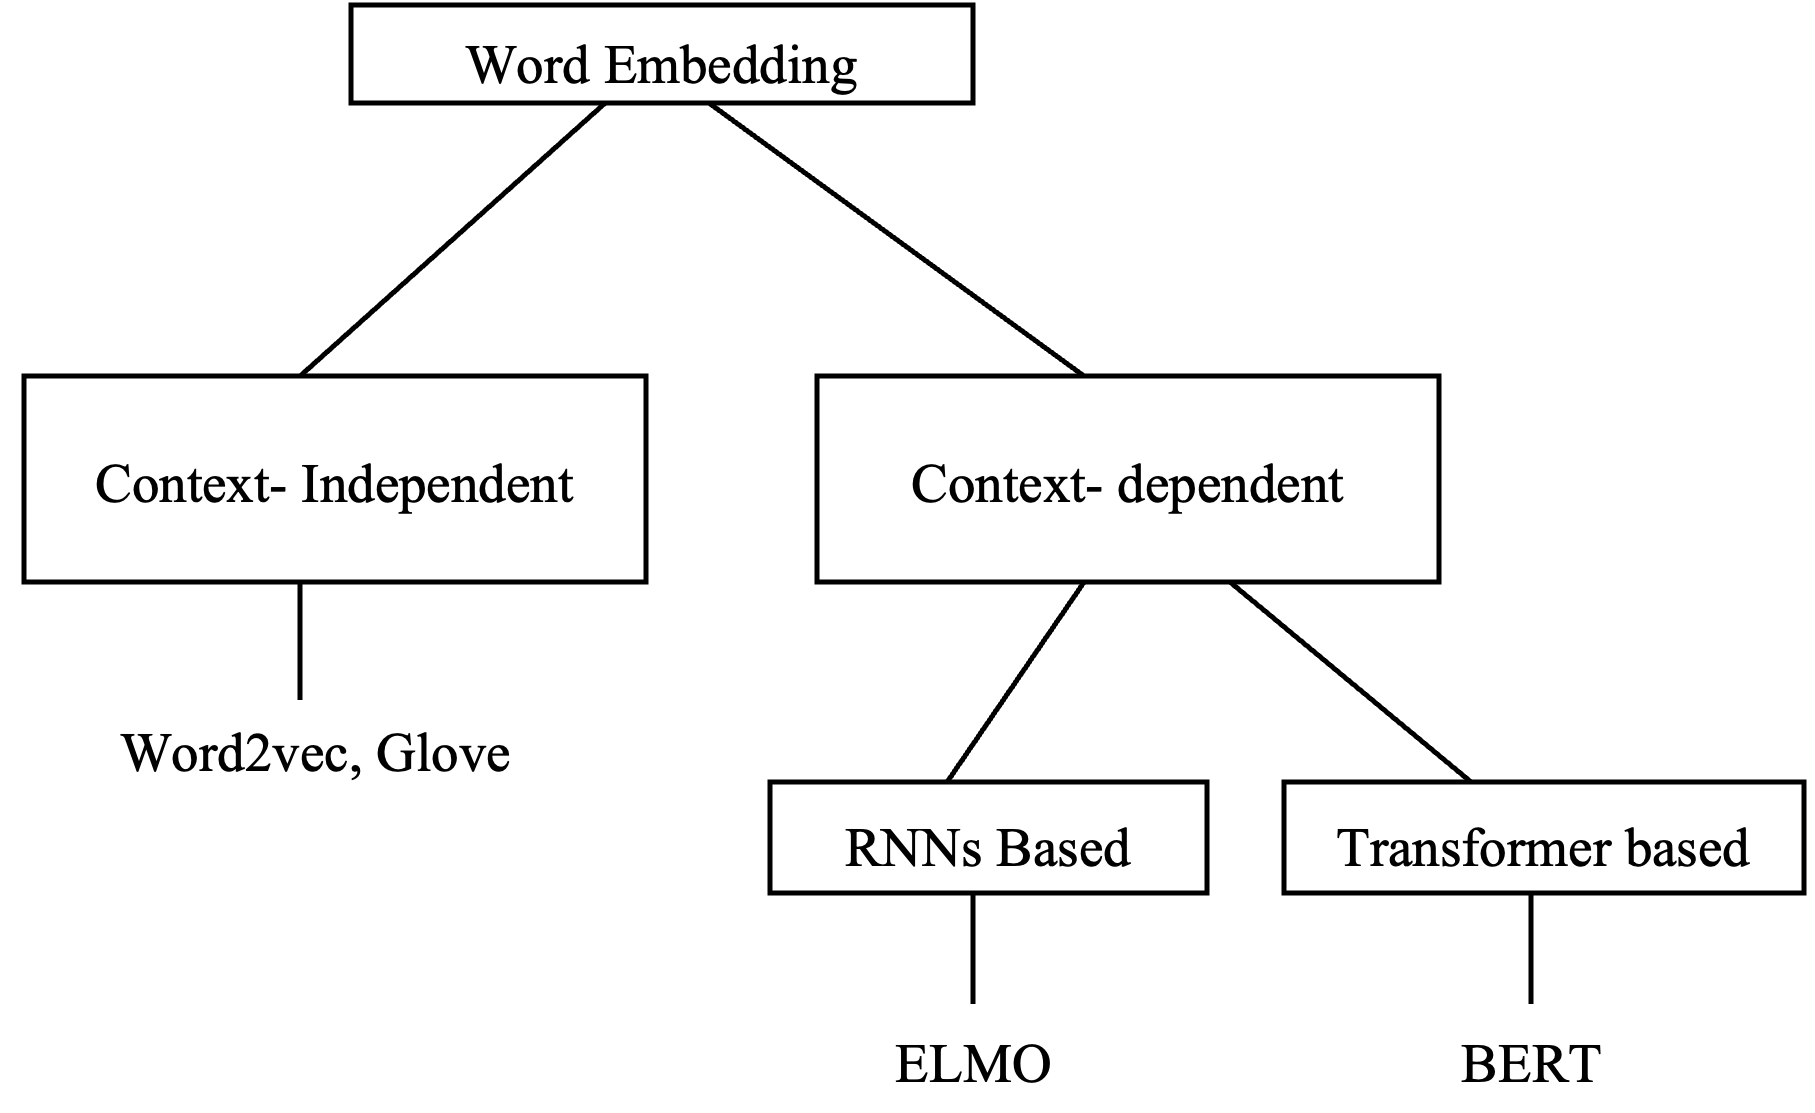
\includegraphics[width=10cm]{images/intro.png}\\
  \caption{A taxonomy of word embedding} 
  \label{fig:taxonomy}
\end{figure}
Finding such representation for words and sentences has been one hot topic over the last few years in the field of Natural Language Processing and has led to many improvements in core NLP task.
This seminar report seeks to compare the effect of different word representation for the Nepali text classification. Here, Word2vec and ELMO word embedding techniques are used for the analysis purpose these are the two category of word representation technique namely context dependent and context independent show in the figure \ref{fig:taxonomy}. All in all, this transformation has two important beneficial properties that is dimensionality reduction for efficient representation and contextual similarity for expressive representations.\\
The remaining part of this seminar report is organized as follow. Literature reviews to this study are described in Chapter 2. In Chapter 3, have described the proposed methodology. The implementation part is described in Chapter 4. Finally, result and conclusion is included in the chapter 5 and 6 respectively.
\subsection{Problem Statement}
The huge unstructured data in the digital world is one of the reasons where the application of various machine learning techniques is possible. However, the complex morphology of text due to various forms of existing consonants and vowel letters make it difficult in feature extraction from the document. Since the different languages are morphologically rich and complex, natural language processing task such as classification and machine translation has become complex because of inappropriate word embedding techniques.
\section{Objective}
\begin{itemize}

  \item {To implement and analysis context dependent and independent word embedding model.}

  \item {To implement SVM and Random Forest Machine learning algorithms for text classification.}

\end{itemize}
\clearpage
\chapter{LITERATURE REVIEW}
Several machine learning algorithms have been developed for performing the natural language processing task, where word embedding techniques play the significant role. Additi-onally, number of researches have been carried out in this topic, some of these are explained in the following section.\\
In paper \cite{bhoir2017comparative}, the author purposed a comparative analysis of different word embedding models namely continuous bag of words, skip gram, Glove (Global Vectors for word representation) and Hellinger- PCA. Additionally, models were compared on different parameters such as performance with respect to size of training data, basic over-view, and relation of context and target words, memory consumption etc. All in all, the author concluded that Glove is the best model as compared to other models as it is scalable to large corpus and worked well even with small corpus.\\
NPVec1, which consist of 25 SATA word embedding for Nepali language that derived from a large corpus using Glove, Word2Vec, fastText, and BERT is discussed in the paper  \cite{koirala2021npvec1}.  It also provided intrinsic and extrinstic evaluation of these embedding using well established metrices and methods. These models were trained using 279 million word tokens and were the largest embedding ever trained for Nepali language. Macro Precision, Recall and F1 metrics were used for the evaluation of the classification model. On average, the F1 scores for word embedding mod- els exceeded the baseline scores by a margin of 5 percent.\\
The author of the paper \cite{ajose2020performance}, conducted experiments on both classic and contextu-alised word embedding for the purpose of text classification. Moreover, to study the impact of word embedding on different dataset, the author selected four benchmarking classification datasets with varying average sample length for comparing both single-label and multi-label classification tasks. This study recommended that choosing CNN over BiLSTM for document classification dataset, where the context in sequence was not as indicative of class membership as sentence datasets. All in all, the author concluded that contextualized embedding was matched well with BiLSTM for SST-2-like classification datasets, while CNN collaborates well with classic embedding for document dataset like 20NewsGroup.\\
In the paper \cite{fano2019comparative}, the aim of the task was to evaluate system for early risk prediction on the internet, in particular to identify users suffering from eating disorders. In the controlled setting, the author evaluated the performance of three different word representation methods: random indexing, GloVe, and ELMo. The best model in term of F1 score turned out to be a model with GloVe vector as input to the text classifier and multi-layer perceptron.\\
In  paper \cite{ritu2018performance}, discussed the performance of three word embedding models namely, word2vec in tensorflow, word2vec from  Gensim package and FastText model. Additionally, dataset used in this research work contained 521391 unique words to produce the clusters and evaluated their performance in terms of accuracy and efficiency.\\

\chapter{METHODOLOGY}
\section{Methodology}
This seminar report is more focus on feature extraction of Nepali news dataset for the text classification task. Additionally, web scraping process is used for the data collection. The figure \ref{fig:Overall} illustrate the step carry out in this seminar report.
\begin{figure}[H]
	\centering 
	\vspace{10pt}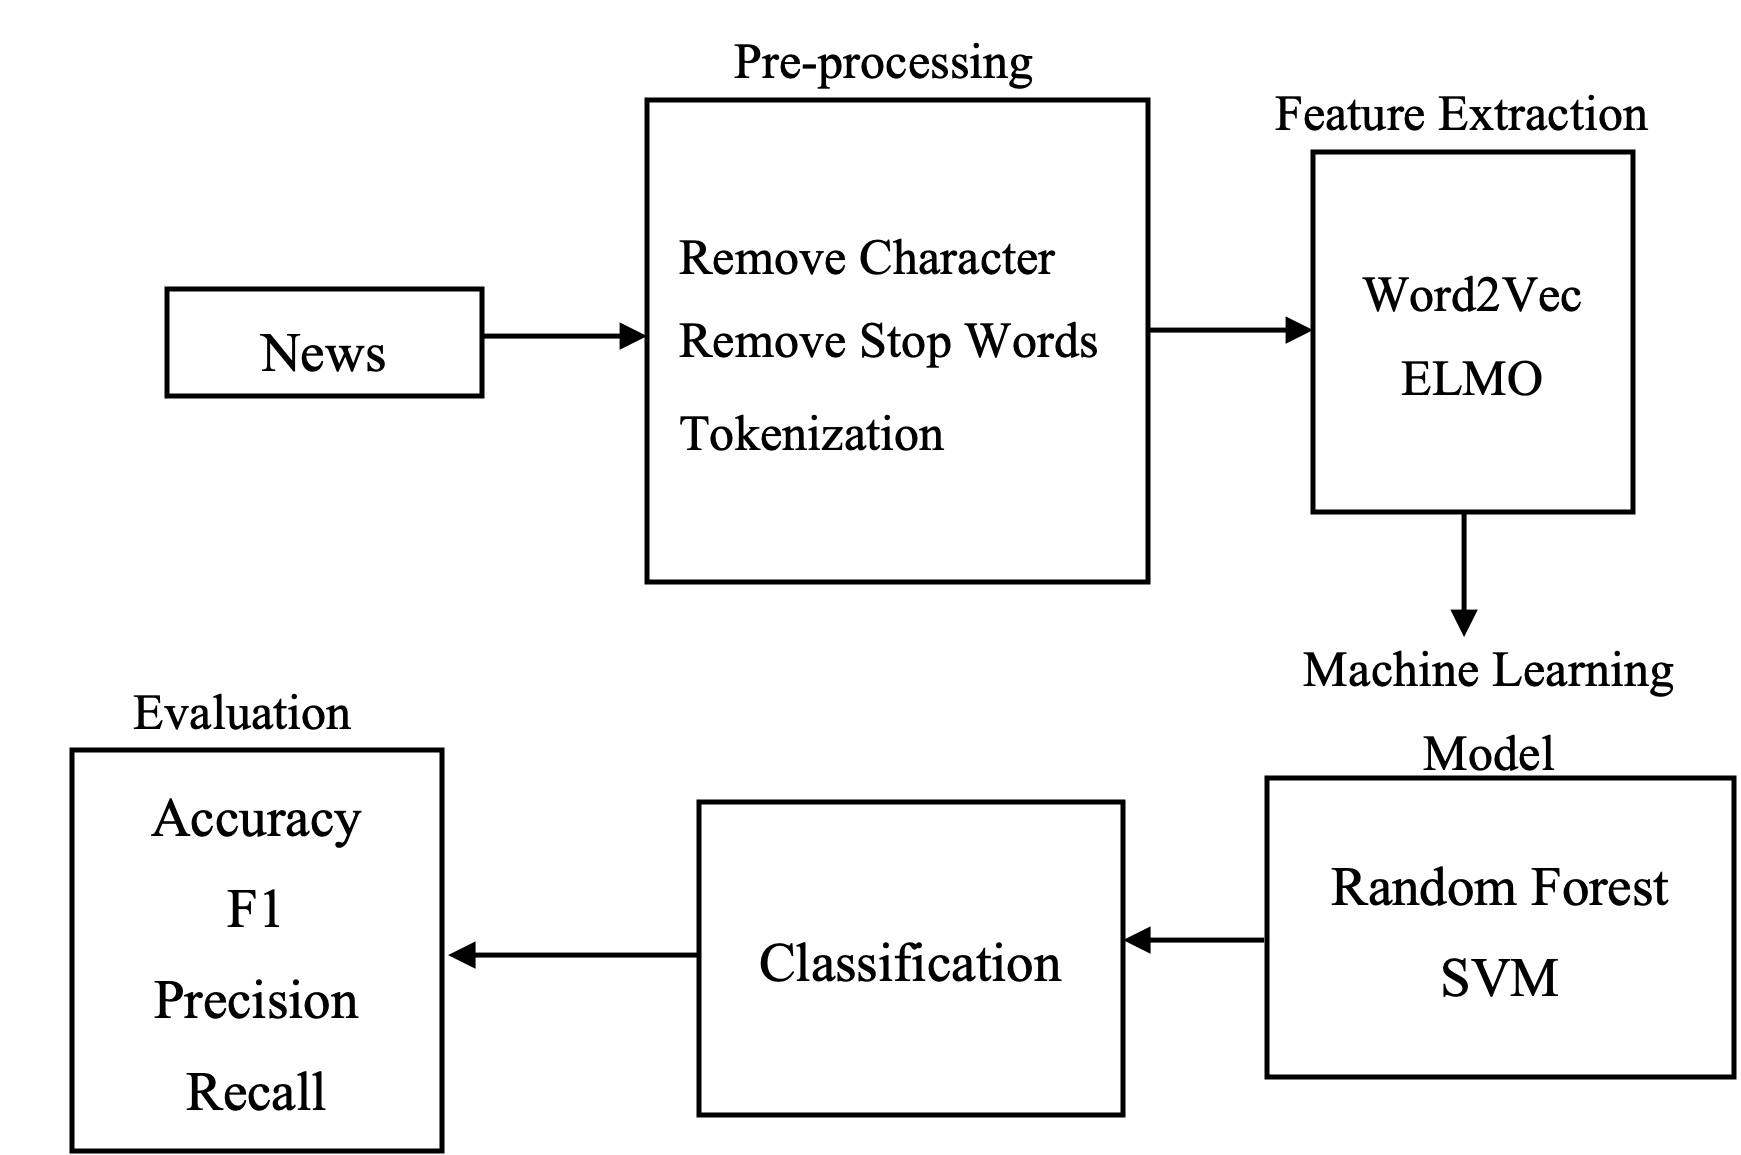
\includegraphics[width=10cm]{images/methodology.png}
	\caption{Overall Process} 
	\label{fig:Overall}
\end{figure}
\section{Dataset Discription}
There are total of 5145 news articles which are scraped from www.ekantipur.com, in four different categories. Categories are Health, National, Opinion, Business. The detail of the dataset is given in the table \ref{table:Dataset}. 
\begin{center}
\begin{table}
\caption{Dataset Description}
\label{table:Dataset}
\centering
\begin{tabular}{ |p{3cm}||p{3cm}|p{3cm}|p{3cm}|  }
 \hline
 Category& Total Data \\
 \hline
 Health   & 1029    \\
 Opinion&   1029  \\
 National &1029\\
 News &1029 \\
 \hline
\end{tabular}
\end{table}
\end{center}
\section{Data Preprocessing}
This step cleans the document by removing HTML tags and noisy characters present in the document, by using different python libraries such as NLTK and regular expression.
\subsection{Remove Special Characters}
Special characters play the negative role in the machine learning algorithm. So, they are removed by using the regular expression library available in the python programming language.
\subsection{Remove Stop Words}
A stop words is a commonly used word that a search engine has been programmed to ignore, both when indexing entries for searching and retrieving them as the result of a search query. Additionally, these data may not play the significant role for the result, so here remove them easily by storing a list of words by considering to be stop words. NLTK (Natural Language Toolkit) in python has a list of stop words stored in 16 different languages.
\subsection{Tokenization}
Tokenization describes splitting paragraphs into sentences, or sentences into individual words. For the former Sentence Boundary Disambiguation (SBD) can be applied to create a list of individual sentences. This relies on a pre-trained, language specific algorithms like the Punkt Models from NLTK. Sentences can be split into individual words and punctuation through a similar process. This seminar report uses tokenization in preprocessing task by using Punkt Models from NLTK.
\section{Feature Extraction}
\subsection{Word2Vec}
Word2Vec is a statistical method for efficiently learning a standalone word embedding from a text corpus. It was developed by Tomas Mikolov \cite{mikolov2013efficient} as a response to make the neural-network-based training of the embedding more efficient then has become the de facto standard for developing pre-trained word embedding. Word2Vec is a method to construct such  embedding. It can be obtained using two methods: Skip Gram and CBOW. The figure \ref{fig:CBOW} show the architecture of CBOW
\begin{figure}[H]
	\centering 
	\vspace{20pt}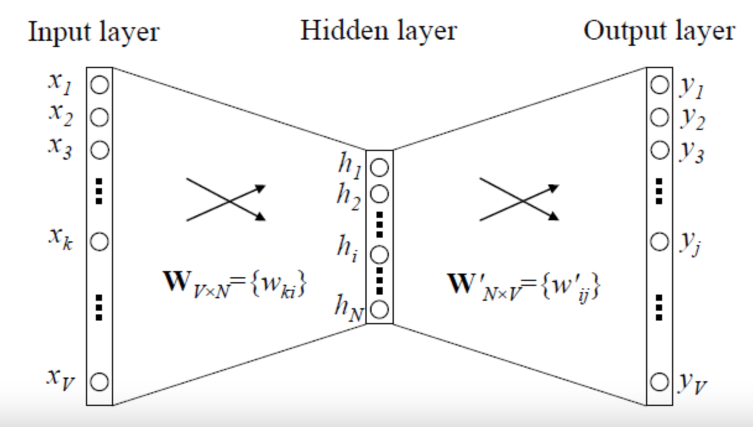
\includegraphics[width=10cm]{images/Word2Vec.png}
	\caption{The CBOW architecture predicts the current word} 
	\label{fig:CBOW}
\end{figure}
Word representations in Word2Vec are taken from a simple neural network, which consists of:
\begin{itemize}
  \item {An input layer}
  \item {A projection layer}
  \item {One hidden layer}
  \item{One output layer}
\end{itemize}
The input is the one hot encoded representation of a word, and the projection layer has dimensionality N*D, while the hidden layer is typically 300 units and learns dense representation. Additionally, the hidden layer has no activation function.
\subsection{ELMo}
The ELMo is a novel way to represent words in vectors or embedding. It was developed by Sarzynska-Wawer, \cite{sarzynska2021detecting}, and these word embeddings are helpful in achieving state-of-the-art (SOTA) results in several NLP tasks such as text classification, machine translation and sentiment analysis.
Unlike most widely used word embedding, ELMo word representations are functions of the entire input sentence. They are computed on top of the two-layer biLMs with character convolution, as a liner function of the internal network state. This setup allows to do semi-supervised learning, where the biLM is pretrained at a large scale and easily incorporated into a wide range of existing NLP architectures. The ELMo architecture is shown in the figure \ref{fig:ELMo}.
\begin{figure}[H] 
	\centering 
	\vspace{20pt}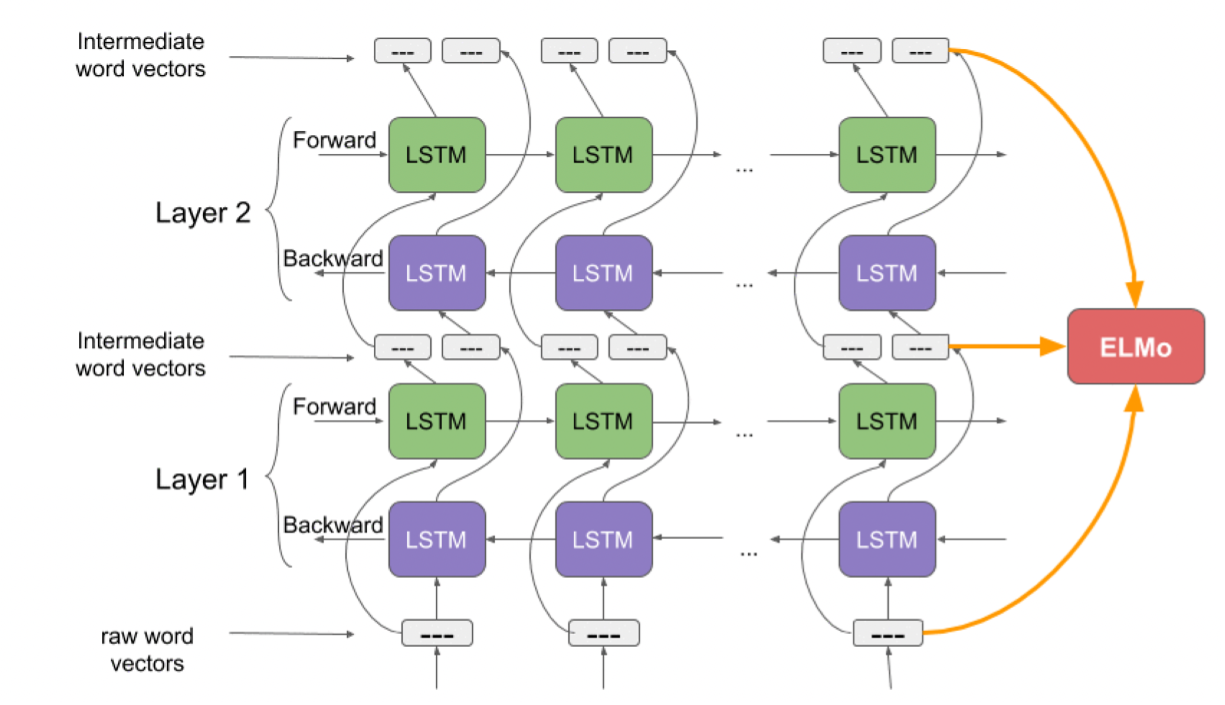
\includegraphics[width=10cm]{images/ELMO.png}
	\caption{Architecture of ELMo}
	\label{fig:ELMo} 
\end{figure}
\section{Machine Learning Model}
\subsection{SVM}
The SVM algorithm is a ‘simple’ linear classification/regression algorithm. It tries to find a hyper plane which separates the data in two classes as optimally as possible. Here as optimally as possible means that as many points as possible of label A should be separated to one side of the hyper plane and as points of label B to the other side, while maximizing the distance of each point to this hyper plane. The hyperplane used in the support vector machine is shown in the figure \ref{fig: SVM_hperplane}.\\
\begin{figure}[H] 
	\centering 
	\vspace{20pt}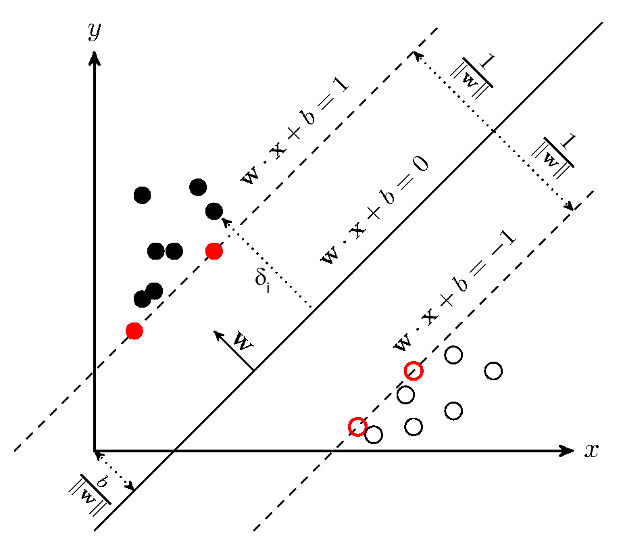
\includegraphics[width=10cm]{images/SVM.png}
	\caption{Support Vector machine hyper plane} 
	\label{fig: SVM_hperplane}
\end{figure}
\textbf{Steps involved in SVM algorithm:}\\
Step 1. Read the training data set. \\
Step 2. Prepared the pattern matrix.\\ 
Step 3. Select kernel function to use. \\
Step 4. Select parameter of the kernel function and value of c \\
Step 5. Execute the training algorithm
\subsection{Random Forest}
Random forest is a supervised machine learning algorithm that is used widely in classificati-on and regression problems. It builds decision tree on different samples and takes their majority vote for classification and average in case of regression. Additionally, one of the most important features of the random forest algorithm is that it can handle the data set containing continuous variable as in the case of regression and categorical variables as in the case of classification.\\
Random forest algorithm is worked on the bagging principal. It is also known as Bootstrap Aggregation is the ensemble technique used by random forest. Bagging chooses random sample from the dataset. Hence each model is generated from the samples provided by the original data with replacement known as row sampling. Additionally, each model is trained independently which generate results. The final output is based on majority voting after combining the results of all models. All in all, the step which involves combining all the results and generating output based on majority voting is known as aggregation. The overall structure of the random forest algorithm is depicted in the figure \ref{fig:random_forest}.\\
\begin{figure}[H] 
	\centering 
	\vspace{20pt}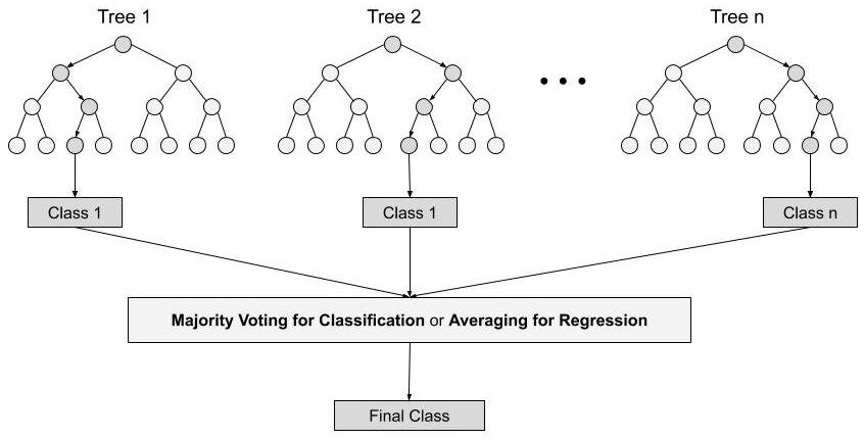
\includegraphics[width=10cm]{images/randomforest.jpg}
	\caption{Random Forest Classifier}
	\label{fig:random_forest} 
\end{figure}
\textbf{Steps involved in random forest algorithm:}\\
Step1: n number of random news are taken from the given dataset.\\
Step2: individual decision trees are constructed for each taken sample news.\\
Step3: each decision tree will generate an output.\\
Step4: final output is considered based on majority voting or average for the news classification
\section{Evaluation Techniques}
\subsection{Accuracy}
In news classification, Accuracy Score is the ratio of correctly predict news classes to the total number of input data points. It can be calculated by using following formula. \
\[ 
 Accuracy=\frac{(TP+TN)}{(TP+FN+TN+FP)} 
\]
Where, \\
TP is the number of True Positive instance\\
FN is the number of False Negative instance\\
FP is the number of False Positive instance\\
TN is the number of True Negative instance
\subsection{Precision}
Precision is the ratio of number of True Positive to the total number of Predicted Positive . It measures out of the total predicted positive, how many are actually positive. All in all, precision score is calculated by using following formula.\
\[ 
 Precision Score=\frac{TP}{(FP+TP)} 
\]
Where,\\
TP is the number of true positive instance\\
FP is the number of false positive instance
\subsection{Recall}
Recall is the ratio of number of True Positive to the total number of Actual Positive. It measures out of the total actual positive, how many are predicted as True Positive, and it can be calculated by using following formula.\
\[ 
 Recall Score=\frac{TP}{(FN+TP)} 
\]
Where,\\
TP is the number of true positive instance.\\
FN is the number of false-negative instance.
\subsection{F1 Score}
It is an important evaluation matric for binary classification that combines Precision and Recall. F1 score is the harmonic mean of precision and recall, whcih is obtained by the following calculation.\
\[ 
 F1 Score=2*\frac{Precision Score*Recall Score}{(Precision Score+Recall Score)} 
\]
\chapter{IMPLEMENTATION}
The implementation include in this seminar report is carried out in the python programming language. Following python libraries are used for the implementation purpose.
\begin{itemize}
  \item {\textbf{Pandas:} pandas is one of the most important libraries of the python programming language, it is used to import the dataset and to obtain the statistical description of the dataset.}
  \item {\textbf{Matplotlib:} This library has been used for plotting graphs. The functions used from this library are as follows: plot(); plot various visualization, show(); to visualize the plots, line(); plot a line graph.}
  \item {\textbf{Sklearn:} This library has been used for splitting the train and test data.}
  \item{\textbf{TensorFlow:} It can be used across a range of task but has a particular focus on training and inference of deep neural network. In this seminar report we use 2.5.3 version of TensorFlow.}
  \item{\textbf{Keras:} It provides a python interface for artificial neural networks. Keras acts as an interface for the TensorFlow library.
  }
\end{itemize}





\section{Data Collection}
Dataset used in this seminar report is collected by performing web scraping process. For this, beautiful soup library is used which is freely available in python programming language. The code snippets for the data collection is depicted in the appendix [A]. 
\section{Preprocessing}
After the data collection process has been completed, the preprocessing task is inaugurated. This process plays a vital role in feature extraction as well as in the machine learning algorithm. It includes different activities such as removing secondary languages, special characters.
\section{Feature Extraction}
Processed data is not directly trained into the machine learning model. In this report, both context dependent and independent techniques are used for converting the text data into the numeric form. Before generating the vector of the data, a news corpus is generated by splitting total word present in the news to a single list and then implement the following techniques.
\subsection{Word2Vec}
The Word2Vec word embedding module is loaded by using genism library available in the python programming language. Additionally, this model only supports the tokenized words so, news is tokenized before passing into it. All in all, different hyperparameters such as size, window size, minimum counts etc., need to be pass for the training process. The code snippets for training this model is depicted in the appendix [B]. 
\subsection{ELMo}
The ELMO model is introduced by Google. It is a pretrained model which is loaded by the help of TensorFlow hub library. Then the preprocessed data is passed for training. Moreover, because of inefficient of computational resources such as Ram, data is divided by taking a window size 20. This model works based on LSTM, so it takes a little bit more time for training as compared to others module. The code snippets for training this model is depicted in the appendix [C]. 
\section{Model Develop and Train}
In this seminar report, SVM and Random forest machine learning algorithms are used for the analysis purpose. These models are loaded from the sklearn library available in python programming language. Additionally, sigmoid kernel is used for classifying the data in SVM. The preprocessed dataset is splitted into train and test in 8:2 ratio for training the model.
\section{System Specification}
The experiment is carried out in the machine with following specifications:\
\begin{itemize}
  \item{\textbf{Processor}: Apple Chip M1}
    \item{\textbf{Ram}: 8 GB}
      \item{\textbf{System Type}: MacOS Monterey}
        \item{\textbf{No of Cores}: 8}
          \item{\textbf{No of Threads}: 4}
\end{itemize}
\chapter{RESULT AND ANALYSIS}
The result of the seminar report is to analysis word embedding models based on news classification. For getting the result, number of pre-processing tasks is performed which is explained in the following section.
\section{Preprocessing}
After data collection process is completed, this is not directly supplied into machine learning algorithm so, some preprocessing tasks need to be performed such as removing stop word, special character and identifying most frequent word etc. The sample of raw news is shown in the figure \ref{fig: Raw_dataset}.
\begin{figure}[H]
	\centering 
	\vspace{20pt}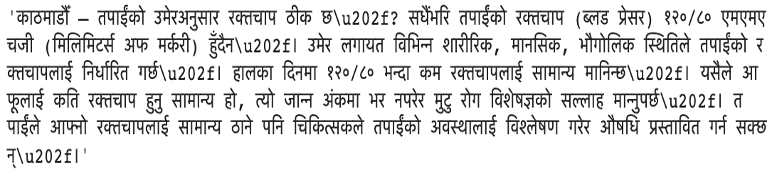
\includegraphics[width=10cm]{images/preprocessing1.png}
	\caption{Sample of Raw Dataset} 
	\label{fig: Raw_dataset}
\end{figure}
Stop words are removed by using the list of stop-words available in NLTK library. Additionally, some special characters are also removed from the raw dataset. All in all, stemming and lemmatization is not performed with these raw datasets. Dataset after completing preprocess is shown in the given figure \ref{fig:Processed_dataset}.
\begin{figure}[H] 
	\centering 
	\vspace{20pt}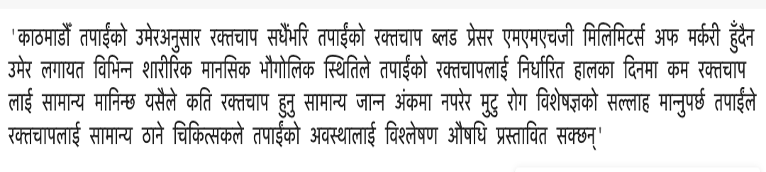
\includegraphics[width=10cm]{images/preprocessing2.png}
	\caption{Sample Preprocess Dataset} 
	\label{fig:Processed_dataset}
	
\end{figure}
\section{Time Performance Analysis}
After the preprocessing task is completed, both Word2vec and ELMO modules are run with varying hyperparameter for the comparative analysis. Additionally, the time stamp required for training each of the models is captured. 
\subsection{Word2Vec}
Here Word2vec model is trained with the processed data for fixed number of features and window size but having different minimum count values. By this analysis it is concluded that this model is trained comparatively fast for minimum count 3 as compared to others. The calculated data are tabulated in the table \ref{table:Word2Vec_minimum_count}
\begin{center}
\begin{table}[H]
\caption{Time Taken by Word2Vec for different minimum count}
\label{table:Word2Vec_minimum_count}
\centering
\begin{tabular}{ |p{4cm}|p{2cm}|p{2cm}|p{2cm}|p{2cm}|  }
 \hline
 Number of Features & 200 &200 &200 &200  \\
 \hline
 Minimum Count   & 1 &2 &3 &4    \\
 \hline
 Window Size &5 &5 &5 &5 \\
 \hline
 Training Time(Second) &77 &59 &49 &50 \\
 \hline
\end{tabular}
\end{table}
\end{center}
The above calculation is visualized in the form of line graph, and which is displayed in the figure \ref{fig:fixed_window_word2vec}.
\begin{figure}[H]
	\centering 
	\vspace{20pt}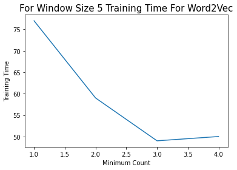
\includegraphics[width=10cm]{images/Word2Vec_fixed_window_line.png}
	\caption{For fixed window size training time for Word2Vec} 
	\label{fig:fixed_window_word2vec}
\end{figure}
Now, here train the same model with same training dataset for various window size, Training time is unexpectedly raised while expanding the window size. The numerical estimates are tabulated in table \ref{table:Minimum_word_word2vec} .
\begin{center}
\begin{table}[H]
\caption{For Fixed Minimum Count Training time for Word2Vec}
\label{table:Minimum_word_word2vec}
\centering
\begin{tabular}{ |p{4cm}|p{2cm}|p{2cm}|p{2cm}|p{2cm}|  }
 \hline
 Number of Features & 200 &200 &200 &200  \\
 \hline
 Minimum Count   & 1 &1 &1 &1    \\
 \hline
 Window Size &4 &8 &10 &12 \\
 \hline
 Training Time(Second) &67 &113 &133 &153 \\
 \hline
\end{tabular}
\end{table}
\end{center}
\subsection{ELMo}
Here ELMO model is trained with the processed data for fixed number of features. By this analysis it is concluded that this model takes longer time for training as compared to Word2Vec. This model takes 1 hours and 36 minutes for generating word embedding vector of preprocessing data. The calculation is depicted in the table \ref{table:training_time_for_ELMO} below.
\begin{center}
\begin{table}[H]
\caption{Training time for ELMO}
\label{table:training_time_for_ELMO}
\centering
\begin{tabular}{ |p{4cm}|p{6cm}|  }
 \hline
 Number of Features & 200 \\
 \hline
 Training Time  & 1 hour 36 minutes    \\
 \hline
\end{tabular}
\end{table}
\end{center}
\section{Model Evaluation}
\subsection{SVM}
For Word2Vec performance of the SVM model is remained constant while increasing the window size. Additionally, it gives maximum of 68 test accuracy for window size equal to eight. Different window size’s values are tabulated in the table \ref{table:SVM_model_accuracy_diff_window_size}.
\begin{center}
\begin{table}[H]
\caption{SVM Model Accuracy for Word2vec with Different Window Size}
\label{table:SVM_model_accuracy_diff_window_size}
\centering
\begin{tabular}{ |p{4cm}|p{2cm}|p{2cm}|p{2cm}|p{2cm}|  }
 \hline
 Number of Features & 200 &200 &200 &200  \\
 \hline
 Minimum Count   & 1 &1 &1 &1    \\
 \hline
 Window Size &4 &8 &10 &12 \\
 \hline
 Model Accuracy &67 &68 &68 &68 \\
 \hline
\end{tabular}
\end{table}
\end{center}
The above calculation is visualized in the form of bar graph and which is displayed in the figure \ref{fig:bargraph_SVM_model_accuracy_diff_window_size}.
\begin{figure}[H]
	\centering 
	\vspace{20pt}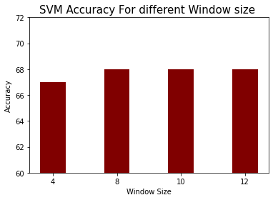
\includegraphics[width=10cm]{images/SVM_accuracy_for_different_window.png}
	\caption{SVM Model Accuracy for Word2vec with Different Window Size} 
	\label{fig:bargraph_SVM_model_accuracy_diff_window_size}
\end{figure}
Here Support Vector Machine Learning algorithm again train with the same dataset for various minimum count. This model showing slight fluctuation behavior while increasing the minimum count to 2,3,4 and so on. This model gives the highest of 67 percent test accuracy on odd number of minimum counts in our sample count. Finally, different test accuracy on different minimum count is tabulated in the table \ref{table: SVM_model_accuracy_diff_minimum_count}.
\begin{center}
\begin{table}[H]
\caption{SVM Model Accuracy for Word2vec with Different Minimum Count}
\label{table: SVM_model_accuracy_diff_minimum_count}
\centering
\begin{tabular}{ |p{4cm}|p{2cm}|p{2cm}|p{2cm}|p{2cm}|  }
 \hline
 Number of Features & 200 &200 &200 &200  \\
 \hline
 Minimum Count   & 2 &3 &4 &5    \\
 \hline
 Window Size &8 &8 &8 &8 \\
 \hline
 Model Accuracy &67 &66 &67 &66 \\
 \hline
\end{tabular}
\end{table}
\end{center}
The above calculation is visualized in the form of bar graph and which is displayed in the figure \ref{fig:bargraph_SVM_model_accuracy_diff_minimum_count}.

\begin{figure}[H]
	\centering 
	\vspace{20pt}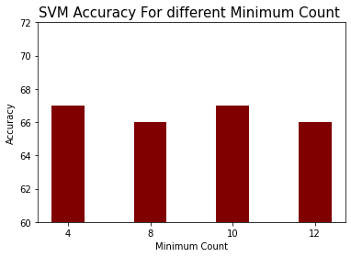
\includegraphics[width=10cm]{images/SVM_accuracy_for_different_minimum_count.png}
	\caption{SVM Model Accuracy for Word2vec with Different Minimum Count} 
	\label{fig:bargraph_SVM_model_accuracy_diff_minimum_count}
\end{figure}
In this seminar report ELMo Word embedding model is also used for the analysis. Because of insufficient of the computational resources, this model is only trained by taking features size of 20. Support Vector Machine learning algorithm gives similar accuracy of 67 percent for the ELMo vectorization as compared to Word2Vec. The detailed classification report of SVM by using ELMO word embedding is shown in the figure \ref{fig:SVM_classification_ELMo}.
\begin{figure}[H]
	\centering 
	\vspace{20pt}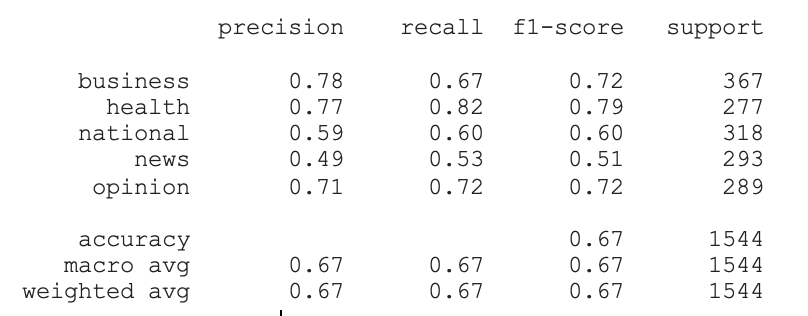
\includegraphics[width=10cm]{images/ELMO_for_SVM.png}
	\caption{SVM Classification Report for ELMO Word embedding} 
	\label{fig:SVM_classification_ELMo}
\end{figure}

\subsection{Random Forest}
For Word2Vec performance of the Random Forest model is increased slightly as compared to the SVM model. For taking 200 features and a single count this model gives the highest of 73 percent test accuracy on window size 4. The data are presented in the table \ref{table:Random_forest_word2vec_diff_window_size}.
\begin{center}
\begin{table}[H]
\caption{Random Forest Model Accuracy for Word2vec with Different Window Size}
\label{table:Random_forest_word2vec_diff_window_size}
\centering
\begin{tabular}{ |p{4cm}|p{2cm}|p{2cm}|p{2cm}|p{2cm}|  }
 \hline
 Number of Features & 200 &200 &200 &200  \\
 \hline
 Minimum Count   & 1 &1 &1 &1    \\
 \hline
 Window Size &4 &8 &10 &12 \\
 \hline
 Model Accuracy &73 &70 &70 &71 \\
 \hline
\end{tabular}
\end{table}
\end{center}
The above calculation is converted into the form of  bar graph which is depicted in the \ref{fig:Randomforest_acccuracy_different_windowsize}.
\begin{figure}[H]
	\centering 
	\vspace{20pt}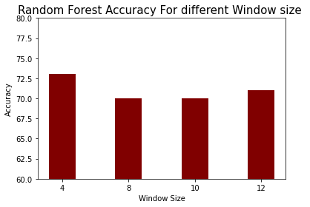
\includegraphics[width=10cm]{images/Randomforest_acccuracy_different_windowsize.png}
	\caption{Random Forest Model Accuracy for Word2vec with Different Window Size} 
	\label{fig:Randomforest_acccuracy_different_windowsize}
\end{figure}
For varying number of minimum counts and constant number of features and window size. The model accuracy is plummeted noticeably. Finally, different test accuracy on different minimum count is tabulated in the table \ref{table:SVM_model_different_minimum_count}.
\begin{center}
\begin{table}[H]
\caption{SVM Model Accuracy for Word2vec with Different Minimum Count}
\label{table:SVM_model_different_minimum_count}
\centering
\begin{tabular}{ |p{4cm}|p{2cm}|p{2cm}|p{2cm}|p{2cm}|  }
 \hline
 Number of Features & 200 &200 &200 &200  \\
 \hline
 Minimum Count   & 1 &2 &3 &4    \\
 \hline
 Window Size &4 &4 &4 &4 \\
 \hline
 Model Accuracy &73 &71 &71 &71 \\
 \hline
\end{tabular}
\end{table}
\end{center}
The above calculation is depicted in the figure .
\begin{figure}[H]
	\centering 
	\vspace{20pt}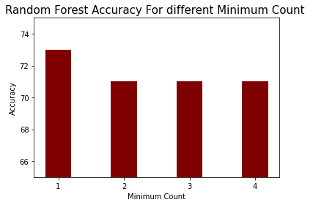
\includegraphics[width=10cm]{images/Random_forest_accuracy_for_different_minimum_count.png}
	\caption{Random Forest Model Accuracy for Word2vec with Different Window Size} 
	
\end{figure}
The word embedding value generated by the ELMO is also used for training the random forest machine learning algorithm. For this embedding random forest gives slightly higher accuracy as compared to the ELMO, it secures 74 percent test accuracy for the news classification system. All in all, classification report is shown in the figure \ref{fig:Random_forest_for_ELMo}.
\begin{figure}[H]
	\centering 
	\vspace{20pt}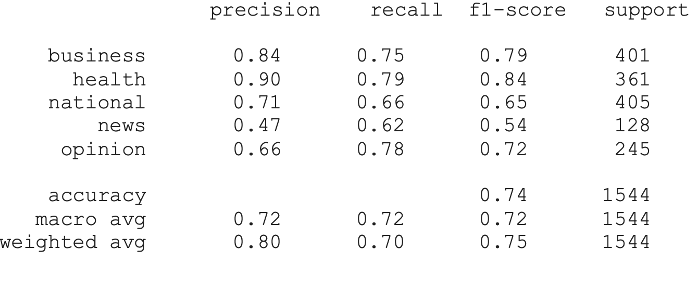
\includegraphics[width=10cm]{images/Random_forest_for_ELMO.png}
	\caption{Random Forest Classification Report for ELMO Word embedding} 
	\label{fig:Random_forest_for_ELMo}
\end{figure}

\chapter{CONCLUSION}
Comparative analysis between different word embedding model is done in this seminar report. The goal of the task is to evaluate system for the Nepali news classification. So, this report evaluated the different word representation methods in the framework of a controlled task. Nepali is a complex language with a wide range of vocabulary containing many rare words.
Language structure use of complex words, multiple meaning in different context all these reasons make it difficult to choose one model as the best for Nepali word classification. Additionally, the content of the dataset also plays the vital role in deciding this.\\
The two word embedding techniques, Word2Vec and ELMO as well as two machine learning algorithms namely SVM and Random Forest are used for the comparative study for the Nepali text classification. Additionally, the dataset for this study is managed by web scraping process. As this report evaluation shows, the model with ELMO vector slightly caught up and surpassed the model with Word2Vec, obtaining higher test accuracy.\\
It is also observed that using Random Forest to classify news led to the high-test accuracy as well as precision and recall as compared to the classification report generated by the Support Vector Machine learning algorithm. However, this model gives the slight balanced classification report.\\
Contrary to the expectation to this seminar, contextualized ELMo vectors did not result in notable performance gain compared to regular Word2Vec model. This could be in part since the stemming with the Nepali text is not easily done in this time. However, increasing the size of dataset and the big overhead in training and testing time for the ELMo model could improve the results.





\renewcommand{\bibname}{References}
\bibliographystyle{plain}
\bibliography{References}

\addcontentsline{toc}{chapter}{\numberline{} References}%
\clearpage
\textbf{\LARGE Appendix}\\[0.5cm] 
\begin{figure}[H]
	\centering 
	\vspace{5pt}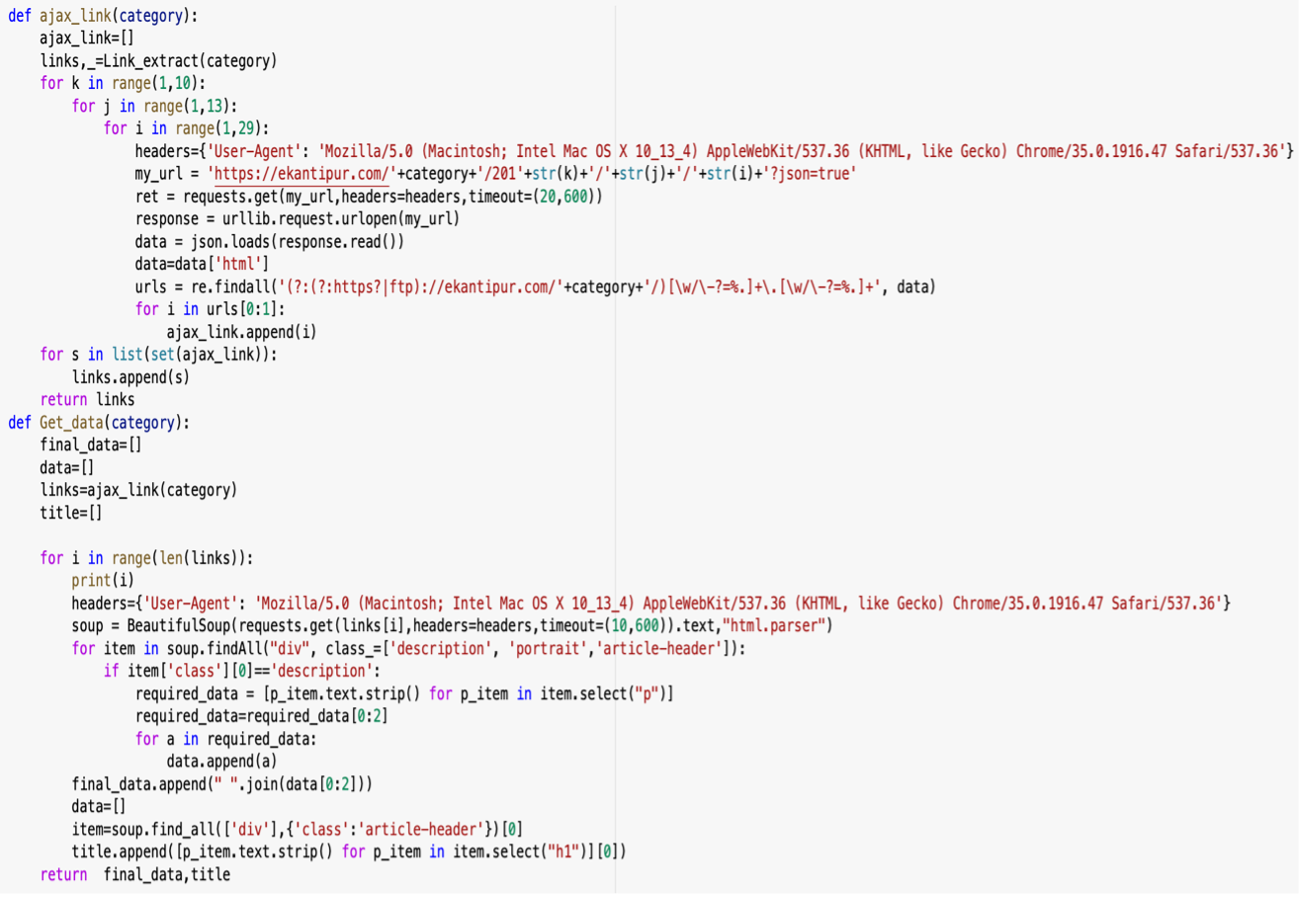
\includegraphics[width=15cm]{images/Data_scrap.png}
\end{figure}
\centering 
[A] Code snippet for Scraping Data.
\begin{figure}[H]
	\centering 
	\vspace{5pt}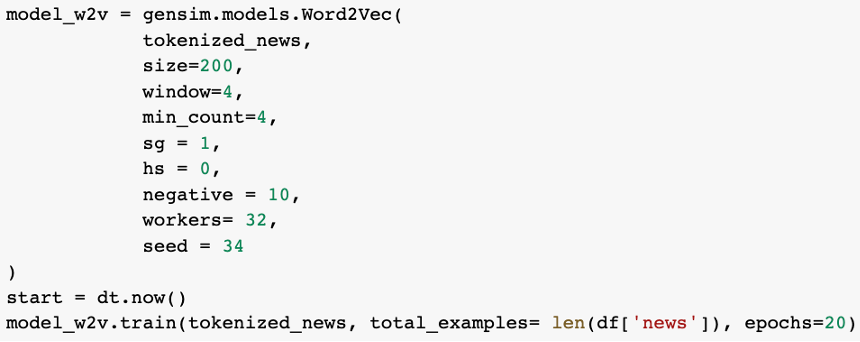
\includegraphics[width=15cm]{images/Word2Vec_model_train.png}
\end{figure}
\centering 
[B] Code snippet for Word2Vect model training.
\begin{figure}[H]
	\centering 
	\vspace{5pt}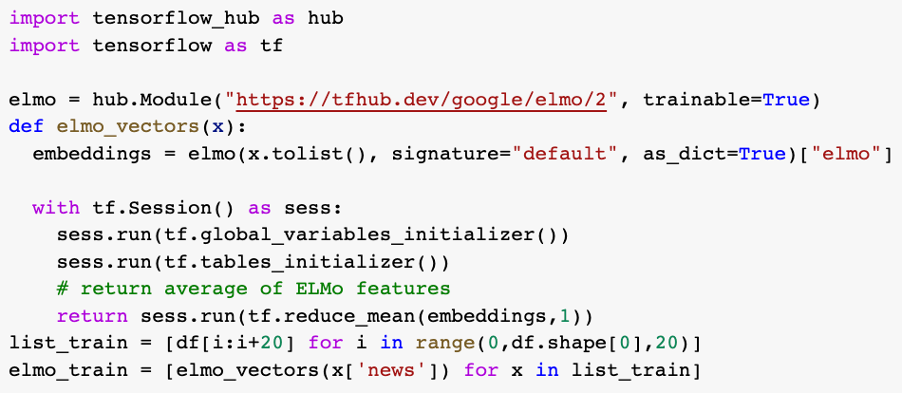
\includegraphics[width=15cm]{images/ELMO_model_train.png}
\end{figure}
\centering 
[B] Code snippet for ELMO model training.
\begin{figure}[H]
	\centering 
	\vspace{5pt}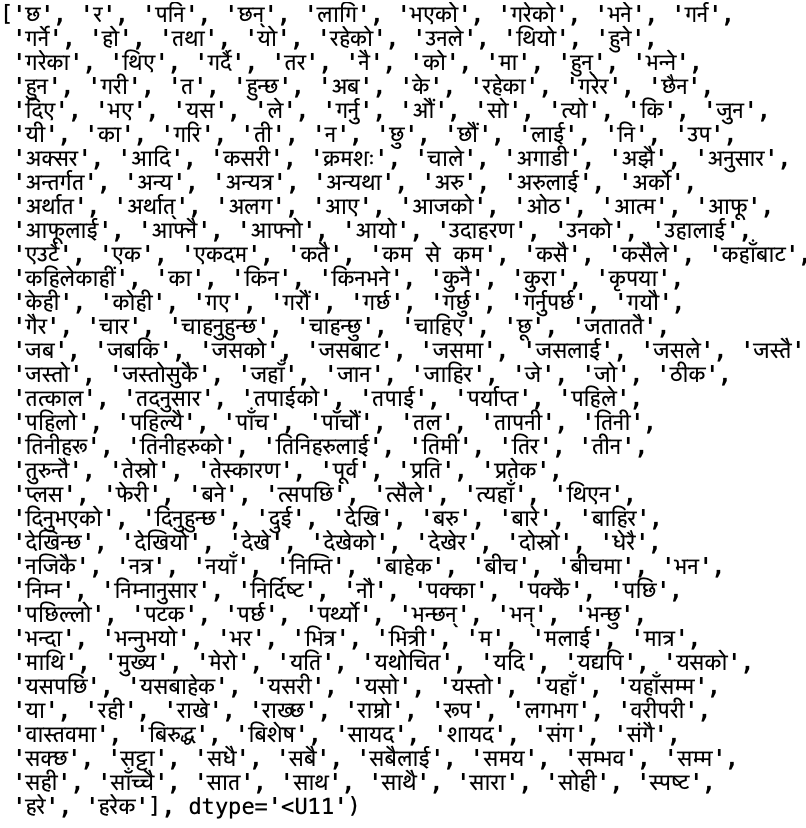
\includegraphics[width=15cm]{images/Stop_words.png}
\end{figure}
\centering 
[C] List of Stop Words

\addcontentsline{toc}{chapter}{\numberline{} Appendix}%

\end{document}